\documentclass[main.tex]{subfiles}
\begin{document}
\begin{titlingpage}
\begin{center}

~ \\[3cm]

%\includegraphics[width=0.6\textwidth]{figurer/ASE}~\\[1cm]

\textsc{\LARGE Bilag 2}\\[1.5cm]

%\textsc{\Large Sundhedsteknologi}\\
%\textsc{\Large 3. semesterprojekt}\\[0.5cm]

\noindent\makebox[\linewidth]{\rule{\textwidth}{0.4pt}}\\
[0.5cm]{\Huge Analyse}
\noindent\makebox[\linewidth]{\rule{\textwidth}{0.4pt}}
\end{center}
\vfill
\begin{center}
{\large 19. december 2017}
\end{center}
\end{titlingpage}

\newpage
\tableofcontents*
\newpage

\chapter{Indledning}


I afsnittet analyse vil der blive beskrevet de overvejelser om mulige løsninger i projektet og hvilke der har valgt at gå videre og begrundelse herom. Der vil blive beskrevet og diskkuteret valget af hardware- og software komponenter som er kritiske for systemet. 


\begin{figure}[H]
\centering
{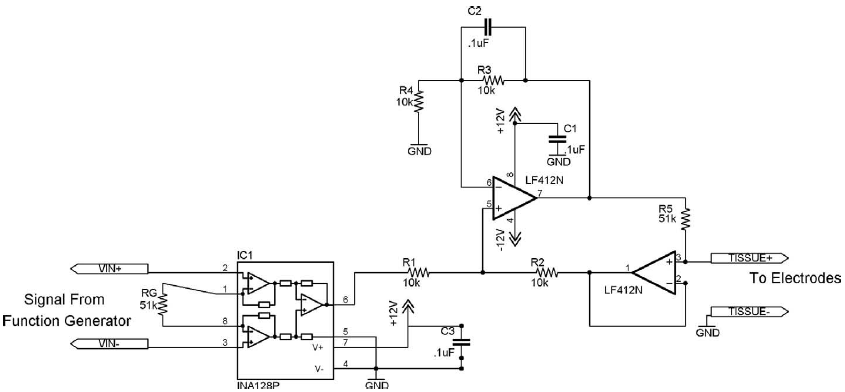
\includegraphics[width=\linewidth]
{Figure/BIdiagram}}
\caption{BI diagram\cite{Aroom2009}}
\label{trefaser}
\end{figure}



\chapter{Hardware}
\section{Bioimpedance}
\subsection{Elektroder}
\subsection{Strømgenerator}
\subsection{Forstækning}
\subsection{Ensretter}
\subsection{Anti-alisering}
\section{EMG}
\section{Analog Discovery}

\chapter{Software}
\section{Waveforms}
\section{Matlab}

\chapter{Konklusion}

\bibliography{Mendeley.bib}
\end{document}


